\subsection{Edmonds' Blossom Algorithm}

The Blossom Algorithm \cite{edmonds1965paths} is an algorithm for finding maximum matching in general graphs. Given a graph $G = (V, E)$, the algorithm finds a matching $M$ such that each vertex in $V$ is incident with at most one edge in $M$ and $|M|$ is maximized.

%\vspace{1em}

\textbf{Motivation} As we learned before, bipartite graphs are a special case, where Matching problem can be efficiently solved. Unfortunately, proposed algorithms do not produce solutions (optimal solutions of the Cardinality Matching or the correct solutions of the Maximum Cardinality Matching) when applied to general graphs. Without further speculations about complexity of both general and special cases, we can pose the following question: What property of bipartite graphs is lost and cannot be utilized, when the problem is loosened to the general case?

\begin{figure}
	\centering
	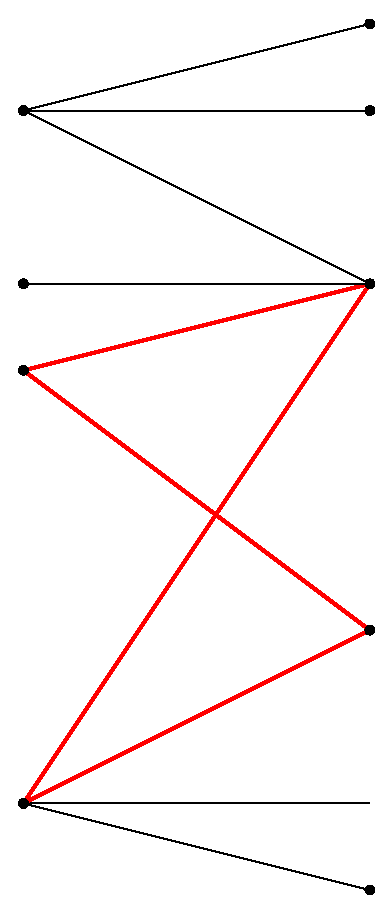
\includegraphics[height=0.4\textwidth]{img/bipartite-even-cycle.eps}
	\caption{Bipartite graphs can have cycles, but only of even length}
	\label{fig:bipartite-even-cycle}
\end{figure}

\begin{figure}
	\centering
	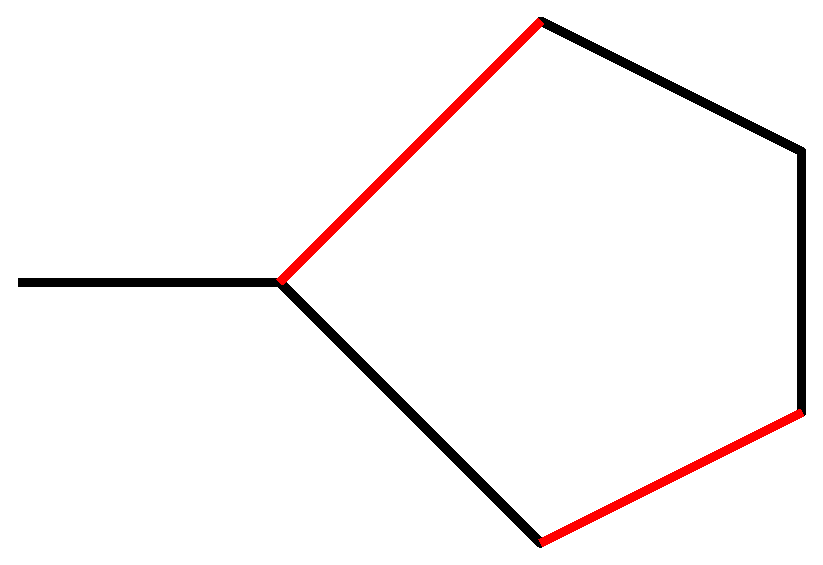
\includegraphics[height=0.2\textwidth]{img/odd-matching-maximal.eps}
	\hspace{2em}
	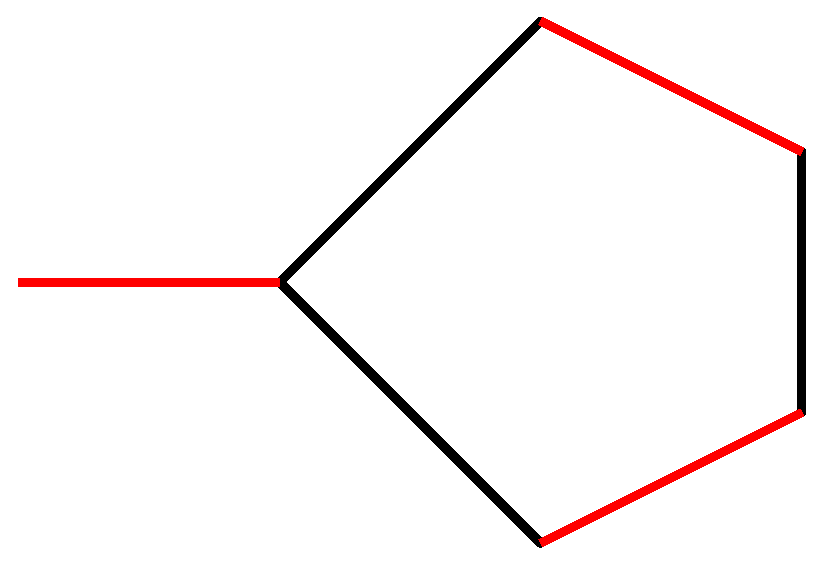
\includegraphics[height=0.2\textwidth]{img/odd-matching-optimal.eps}
	\caption{Maximal: matching of size 2, optimum: matching of size 3}
	\label{fig:maximal-optimal-cycle}
\end{figure}

\textbf{Observation} One of the benefits of having graph's edges only between two disjoint (sub)sets of vertices is that all possible cycles in the graph are of the even length (Fig. \ref{fig:bipartite-even-cycle}). If the cycle has an odd length, it is possible that (for example, greedy-generated) solutions will be sub-optimal (Fig. \ref{fig:maximal-optimal-cycle}).

Blossom algorithm uses the idea of Berge’s Theorem \cite{berge1957two}, that
matching is a maximum matching iff there is no augmenting path.
It takes Graph $G$, initial matching $M$ on $G$ as \textit{input} values and produces maximum matching $M^*$ on $G$ as \textit{output}. Starting from an initial matching, the algorithm computes a maximum matching by augmenting the current matching with augmenting paths as long as it can find them and returns whenever no augmenting paths are left. 

\textbf{Problem} How to guarantee no augmenting paths in a graph?

\begin{definition}
	\textbf{Exposed vertex} Vertex $v$ is exposed iff no edge of $M$ is incident with $v$.
\end{definition}

\begin{definition}
	\textbf{Blossom} B is a cycle in G consisting of 2k+1 edges of which exactly k belong to M, and where one of the vertices v of the cycle (base) is such that there exists an alternating path of even length (stem) from v to an exposed vertex w.
\end{definition}

\begin{definition}
	\textbf{Contracted Graph} G’ the graph obtained from G by contracting every edge of a blossom B into one vertex.
\end{definition}

\begin{figure}
	\centering
	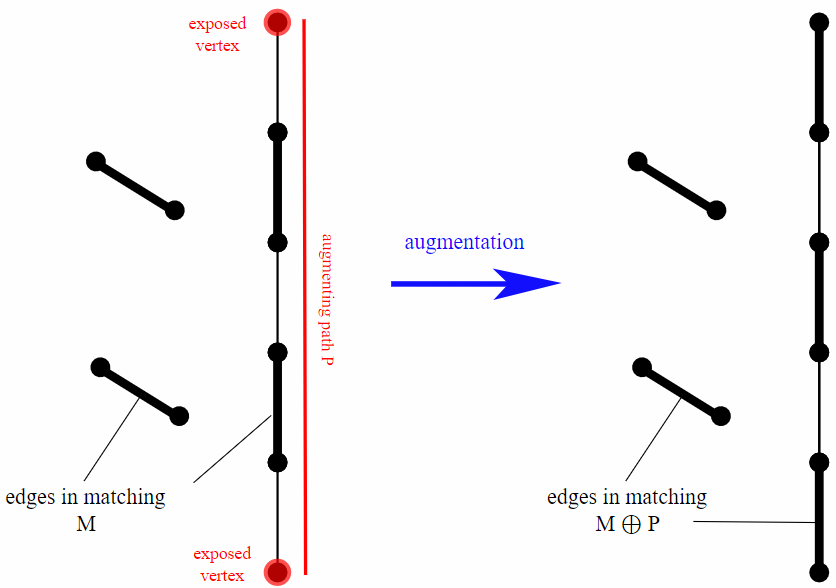
\includegraphics[width=0.75\textwidth]{img/Edmonds_augmenting_path.png}
	\caption{Augmenting a path}
	\label{fig:augmenting-a-path}
\end{figure}

\textbf{Finding an augmenting path} The search for an augmenting path uses an auxiliary data structure consisting of a forest F whose individual trees correspond to specific portions of the graph G. In fact, the forest F is the same that would be used to find maximum matchings in bipartite graphs (without need for shrinking blossoms). In each iteration the algorithm either (1) finds an augmenting path (Fig. \ref{fig:augmenting-a-path}), (2) finds a blossom and recurses onto the corresponding contracted graph, or (3) concludes there are no augmenting paths.

\textbf{Finding Blossoms}
The algorithm traverses the graph starting from an exposed vertex. Computing the set of exposed vertices can be done cheaply by substracting the vertices of $M$ from $G$. Starting from that vertex, it labels it as an outer vertex "o". Then, it alternates the labeling between vertices being inner "i" and outer "o" such that no two adjacent vertices have the same label. If two adjacent vertices are labeled as outer "o" then an odd-length cycle (and therefore a blossom) is found. See Fig. \ref{fig:contracting-a-blossom}.

\begin{figure}
	\centering
	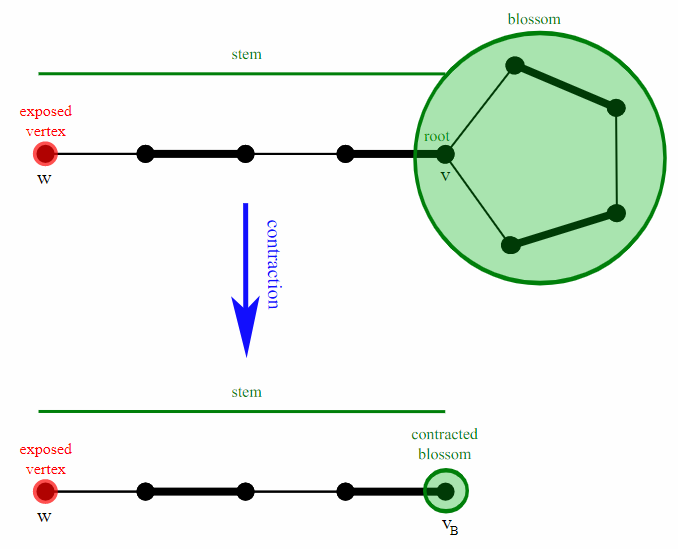
\includegraphics[width=0.75\textwidth]{img/Edmonds_blossom_contraction}
	\caption{Contracting a blossom}
	\label{fig:contracting-a-blossom}
\end{figure}

After finding and contracting a blossom, the algorithm is executed recursively on the contracted graph. For general graphs, a straightforward implementation of the maximum matching algorithm of Edmonds runs in $\mathcal{O}(|V|^4)$ time \cite{papadimitriou1982combinatorial}. However, more efficient algorithms like the one from \cite{micali1980v} which runs in
$\mathcal{O}(\sqrt{|V|}*|E|)$ are known.

